\section{\neupims Scheduling}
\label{sec:scheduler}

The integration of dual row buffers enables \neupims to handle NPU's memory accesses and PIM commands simultaneously.
%
This section describes computation overlapping opportunities for multi-head attention (MHA) layer execution and a novel request scheduling technique for batched LLM inferencing, dubbed \textit{sub-batch interleaving}.

\subsection{Overlapping Opportunities in MHA Layer}
%
\begin{figure}[t]
\centering
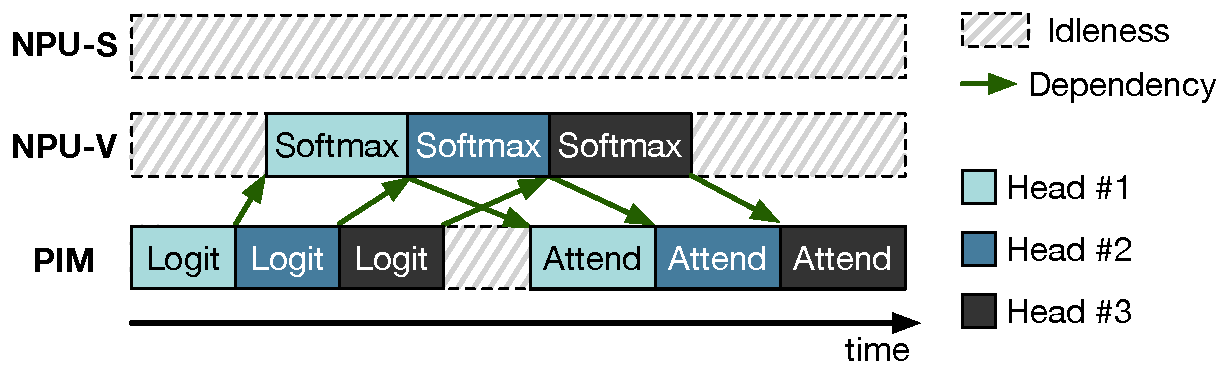
\includegraphics[width=1.0\linewidth]{figure/overlap-mha.pdf}
\vspace{-3ex}
\caption{Overlapping opportunities of multi-head attention layers. NPU-S: systolic arrays; NPU-V: vector units.}
\vspace{-1ex}
\label{fig:overlap-mha}
\end{figure}

\begin{figure}[t]
        \centering
        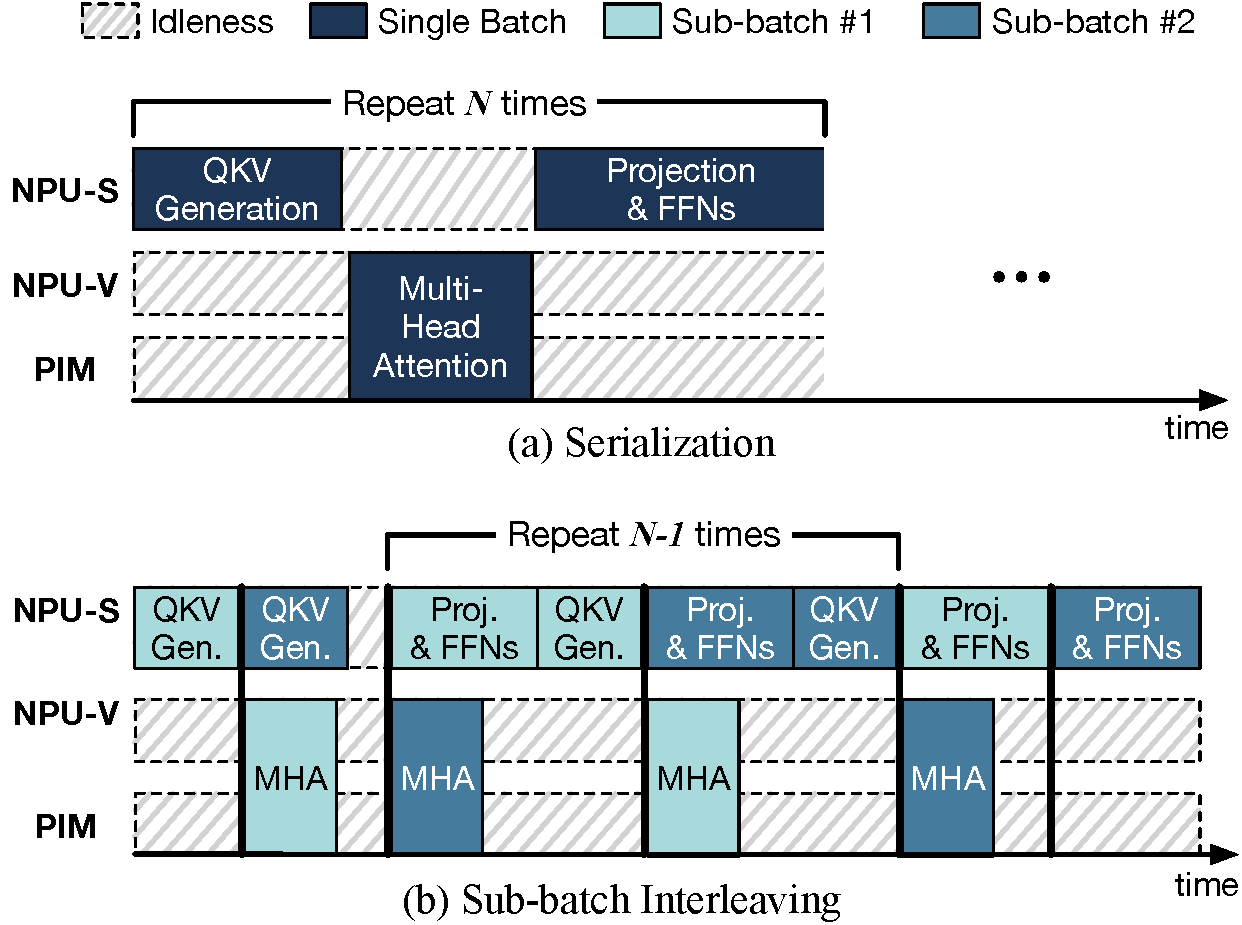
\includegraphics[width=1.0\linewidth]{figure/sub-batch-interleaving.pdf}
        \vspace{-3ex}
        \caption{Example execution timelines of LLM decoder blocks: (a) Serialized execution, (b) Sub-batch interleaving. NPU-S: systolic arrays; NPU-V: vector units; \(N\): the number of decoder blocks.}
        \vspace{-3ex}
        \label{fig:sub-batch-interleaving}
\end{figure}

%
Figure~\ref{fig:overlap-mha} illustrates the overlapping of (1) logit and attend operations on PIM-side, and (2) softmax operations on NPU-side in \neupims.
%
As operations of multi-head attention can be decomposed to a head granularity, even na\"ive NPU-PIM integrated architecture should have an opportunity to harness both resources to overlap operations.
%
However, it cannot take advantage of this opportunity because operational results cannot be transferred between PIM units and vector units through PIM channels.
%
In contrast, \neupims, by employing dual row buffers, can concurrently harness both NPU and PIM.
%
This configuration allows vector units within \neupims to store partial logit (softmax) values without having to wait for the completion of the entire logit operations (GEMV) on the PIM, reducing the underutilization of integrated units.

% %

It is worthwhile to note that this overlapping is only possible because there is head-level parallelism, which is only available within the multi-head attention layer.
%
Further, the overlapping opportunity exists only between PIM and vector units of NPU, resulting in the NPU's systolic arrays largely remaining unused during the execution of the MHA layer.


%
\subsection{Sub-batch Interleaving}
\label{subsec:sub-batch}
%
\niparagraph{Limitation of serialized executions.}
%
Figure~\ref{fig:sub-batch-interleaving}(a) illustrates an example execution timeline of the decoder block operations, running on a na\"ive NPU-PIM integrated device.
%
In particular, the figure depicts the algorithmic dependencies among QKV generation, multi-head attention, and projection \& FFNs, within the batch. 
%
Due to the dependencies, they must be executed serially, inevitably leading to low utilization on both NPU and PIM.  
%

\niparagraph{Interleaving the two sub-batches.}
%
To tackle this challenge, we propose \textit{sub-batch interleaving} that partitions one large batch into two sub-batches and alternate them to improve resource utilization.    
%
Figure~\ref{fig:sub-batch-interleaving}(b) delineates the sub-batch interleaving technique that allows the simultaneous executions of PIM-friendly and NPU-friendly operations within the sub-batches on the PIM and NPU, respectively, significantly improving the utilization of both NPU and PIM.
%
%


\niparagraph{Comparative analysis on the execution timelines.}
%
Let $N$ denote the number of decoder blocks to be executed on a single \neupims device.
%
Figure~\ref{fig:sub-batch-interleaving}(a) shows that without the use of sub-batch interleaving, the operators in each decoder block would be executed sequentially, leading to a total execution time equal to $N$ times the per decoder-block execution time (i.e., QKV generation on NPU-S + MHA on PIM \& NPU-V + Projection \& FFNs on NPU-S). 
%

%
However, as depicted in Figure~\ref{fig:sub-batch-interleaving}(b), sub-batch interleaving effectively hides the execution times of MHA layer in the NPU-S execution times, resulting in the total execution time equal to  ($N$ - 1) times the per-sub-batch partial execution time (i.e., Projection, FFNs, and QKV generation on NPU-S) plus a single decoder-block execution time divided at the start and end.
%
While the interleaving occurs, the NPU and PIM utilization is improved as their executions are effectively overlapped.
%
Our empirical study demonstrates that the \neupims execution time in the interleaved period is mostly bounded by the NPU execution time running GEMM operations, hiding the PIM execution time for MHA layer execution.
%

\niparagraph{Challenges.}
%
For optimal exploitation of parallelism inherent in sub-batch interleaving, \neupims must consider two key aspects:
First, \neupims requires a strategic balancing of the execution time for each sub-batch, particularly focusing on the multi-head attention.
Since the latency of multi-head attention is determined by the channel processing the longest sequence, we must implement load balancing across the channels, ensuring an equitable distribution of token lengths.
This challenge is addressed through a channel load balancing algorithm (Section~\ref{subsec:channel-load-balancing}).
Second, \neupims must ensure similar execution times for both sub-batches for efficient interleaved execution.
The duration of each stage within the interleaving is bound by the processing time of more time-consuming sub-batch.
For that, \neupims introduces a sub-batch partitioning algorithm (Section~\ref{subsec:sub-batch-partition}).

\SetKwInOut{Input}{input}
\SetKwInOut{Output}{output}
\SetKwInput{KwData}{Parameter}
\SetKwComment{Comment}{\textsf{//} }{}
\SetKwComment{CommentTwo}{/* }{~*/}

\begin{algorithm}[tb]
\footnotesize
\caption{MHA Latency Estimation}
\label{alg:estimate-mha}
\LinesNumbered

\KwIn{$
\hspace{0.2em}\quad\quad\ {seq\_len}:\   \small\textit{Sequence length of the request} % {seq\_len}
$}
\KwData{$
\hspace*{0.2em}{E}:\     \small\textit{Model embedding size}\newline
\hspace*{0.2em}{L}_{tile}:\   \small\textit{GEMV latency for one PIM tile} \newline % {L}_{tile}
\hspace*{0.2em}{L}_{GWRITE}:\  \small\textit{GWRITE latency for global buffer} \newline 
\hspace*{0.2em}{E}:\  \small\textit{Model embedding size}\newline
\hspace*{0.2em}{P}_{DRAM}:\  \small\textit{DRAM page size}\newline
\hspace*{0.2em}{B}_{chnl}:\  \small\textit{PIM banks per channel}\newline
\hspace*{0.2em}{N}_{head}:\  \small\textit{Number of heads}
$}
\KwOut{$
\hspace{0.2em} \quad\ \ {L}_{MHA}:\ \small\textit{Estimated latency for MHA}% {L}_{MHA}
$}

\vspace{1ex}
$L_{MHA}\ \leftarrow\ 0$\; \CommentTwo{\textit{\textsf{\footnotesize{\textbf{GEMV latency for \ensuremath{Key^T \times\ Query}}}}}}
$N_{tiles}\ \leftarrow\ ({seq\_len}\ /\ {B}_{chnl})\ *\ (E\ /\ P_{DRAM})$\;
${L}_{MHA}\ +=\ L_{GWRITE}\ *\ (E\ /\ P_{DRAM})$\;
${L}_{MHA}\ +=\ L_{tile}\ *\ N_{tiles}$\;
\vspace{1ex}
\CommentTwo{\textit{\textsf{\footnotesize{\textbf{GEMV latency for \ensuremath{Logits\ \times\ Value}}}}}}
$N_{tiles}\ \leftarrow\ ((E/N_{head})/B_{chnl})*((seq\_len/P_{DRAM})*N_{head})$\;
${L}_{MHA}\ +=\ L_{GWRITE}\ *\ ((seq\_len\ /\ P_{DRAM})\ *\ N_{head})$\;
${L}_{MHA}\ +=\ L_{tile}\ *\ N_{tiles}$\;
\Return{$L_{MHA}$}
\end{algorithm}
\vspace{-1ex}


\subsection{Multi-Head Attention Latency Estimation}
\label{subsec:estimate-mha}
%
The latency of operations running in the NPU is largely dependent on the batch size of the inference. 
%
%
To apply optimization techniques for multi-head attention, we estimate the execution time of its operations by considering the key-value mapping to the PIM memory layout. 
%
Since the vector for GEMV is shared across the banks, the matrix for GEMV is interleaved row-wise to each banks.
%
Consequently, key caches at the same row and column share the same layer and head index, with differing sequence indices. 
%
Conversely, value caches at the same row and column share the same layer, head, and sequence index, interleaving each head embedding into banks. 
%
Algorithm~\ref{alg:estimate-mha} takes this mapping into account to estimate the execution time of the multi-head attention latency.

\SetKwInOut{Input}{input}
\SetKwInOut{Output}{output}
\SetKwInput{KwData}{Parameter}
\SetKwComment{Comment}{\textsf{//} }{}
\SetKwComment{CommentTwo}{/* }{~*/}

\SetKwFunction{GetLoad}{\textnormal{GetLoad}}
\SetKwFunction{Min}{\textnormal{Min}}
\SetKwFunction{append}{\textnormal{append}}
\SetKwFunction{MHAest}{\textnormal{MHALatencyEstimation}}
\SetKwFunction{Index}{\textnormal{index( )}}

\begin{algorithm}[tb]
\footnotesize
% \caption{Channel Load Balancing }
\caption{Greedy Min-Load Bin Packing}
\label{alg:channel-load-balancing}
\LinesNumbered
\KwIn{$
    \hspace{0.25em}{L_{req}}:\ \small\textit{A list for sqeunce length of new requests }\newline 
    \hspace{0.25em}\ \ \ {L_{chnl}}:\ \small\textit{A list for request allocation of channels }
$}
% \KwOut{$
%     \hspace{0.25em}{seq\_len}: \small\textit{A\enspace sequence\enspace length \enspace of \enspace request}
% $}

\vspace{1ex}
\CommentTwo{\textit{\textsf{\small{Calculate each channel's total load by applying \newline MHA latency estimation to each allocated request }}}}
% $L_{load}\ =\ \GetLoad{\ensuremath{L_{channel}}}$\;
$L_{load}\ \leftarrow\ []$\;
\ForEach{$chnl$ in \ $L_{chnl}$}{
    $Sum_{load}\ \leftarrow\ 0$\;
    \ForEach{$req$ in \ $chnl$}{
        $Sum_{load}\ +=\ \MHAest{req}$
    }
    $L_{load}.\append{\ensuremath{Sum_{load}}}$\;
}
\vspace{1ex}
\CommentTwo{\textit{\textsf{\small{Allocate each request by greedy algorithm}}}}
\ForEach{$new\_req$ in \ $L_{req}$}{
    $min\_index\ =\ {\Min{\ensuremath{L_{load}}}.\Index}$\;
    $L_{chnl}[min\_index].{\append{new\_req}}$\;
    $load_{req}\ =\ \MHAest{new\_req}$\;
    $L_{load}[min\_index]\ +=\ {\ensuremath{load_{req}}}$\;
}
\Return{$L_{chnl}$}
\end{algorithm}
\vspace{-1ex}

\subsection{Greedy Min-Load Bin Packing Algorithm.}
\label{subsec:channel-load-balancing}

To minimize the execution time discrepancy between the most
congested channel and the load-free channel, we developed
the channel load balancing algorithm. Algorithm~\ref{alg:channel-load-balancing} leverages
the aforementioned multi-head attention latency estimation
to batch requests. It initially sorts the batch of requests in
decreasing order of input token length. Then, \neupims
places a request with the longest token length in the channel
with minimal load. At each iteration, it updates the estimated
latency, taking into account the newly appended request.

\neupims allocate LLM inference requests to one of the PIM channels.
%
A PIM channel constitutes multiple PIM banks, each of which partially executes the MHA layers of the assigned requests.
%
%
Thus, it is crucial to minimize the execution time discrepancy between the most congested channel and the load-free channel for load-balancing purposes. 
%
To this end, we develop \emph{greedy min-load bin packing algorithm}, as presented in Algorithm~\ref{alg:channel-load-balancing}.
%
This algorithm leverages the aforementioned multi-head attention latency estimation to batch requests. 
%
As implied by its name, the algorithm greedily allocates requests starting from the longest sequence length to the least loaded PIM channel sequentially.
%
Therefore, it initially sorts the batch of requests in decreasing order of input token length. 
%
Then, \neupims places a request with the longest token length in the channel with minimal load. 
%
At each iteration, it updates the estimated latency, taking into account the newly appended request.
%

\SetKwInOut{Input}{input}
\SetKwInOut{Output}{output}
\SetKwInput{KwData}{Parameter}
\SetKwComment{Comment}{\textsf{//} }{}
\SetKwFunction{Size}{\textnormal{Size}}
\SetKwFunction{Ceil}{\textnormal{\textbf{ceil}}}
\SetKwFunction{Floor}{\textnormal{\textbf{floor}}}
\SetKwFunction{append}{\textnormal{append}}


\begin{algorithm}[tb]
\footnotesize
\caption{Sub-Batch Partitioning }
\label{alg:sub-batch-partition}
\LinesNumbered

\KwIn{$
    \hspace{0.25em}\ \ \ {L_{req}}:\ \small\textit{A list of active request set in each channel}
$}

\KwOut{$
    \hspace{0.25em}{SB_1,\ SB_2}:\ \small\textit{Sub-batchs for interleaving}
$}
\vspace{1ex}

% \cancel{$turn\ \leftarrow\ True$\;}
$turn\ \leftarrow\ True$;

$SB_1,\ SB_2\ \leftarrow\ []$\;
\ForEach{$req_{chnl}$ in $L_{req}$}{
        $bsize\ \leftarrow\ \Size{\ensuremath{req_{chnl}}}\ /\ 2$\;

    \If{$\Size{\ensuremath{req_{chnl}}}\ \%\ 2\ !=\ 0$}{
            $bsize\ =\ turn\ ?\ \Ceil{\ensuremath{bsize}}\ :\
            \Floor{\ensuremath{bsize}}$\;

            $turn\ =\ !turn$\;
    }

        $bsize\ =\ \mathbf{int}({\ensuremath{bsize}})$;

    \vspace{1ex}
        $SB_1.\append{\ensuremath{req_{chnl}[:\ bsize]}}$\;
        $SB_2.\append{\ensuremath{req_{chnl}[bsize\ :]}}$\;

    % \magenta{\CommentTwo{\textit{\textsf{\small{Remove: From here}}}}}
    % \If{\cancel{$size\ !=\ 0$}}{
    %     \cancel{
    %     $size\ =\ turn\ ?\ \Ceil{\ensuremath{size}}\ :\
    %      \Floor{\ensuremath{size}}$\;
    %      }
         
    %     \cancel{ 
    %     $turn\ =\ !turn$
    %     }
    % }
    % \magenta{\CommentTwo{\textit{\textsf{\small{Remove: To here}}}}}
}
\Return{$SB_1,\ SB_2$}

\end{algorithm}





% \begin{algorithm}
% \caption{Sub-Batch Partitioning Algorithm}
% \label{alg:sub-batch-partition}
% \begin{algorithmic}[1]
%     \Require A list of request sequence length in channel [$l1, l2, ..., lk$]
%     % \Ensure $y = x^n$
%     \STATE return Two sub-batches
%     \Statex
% \end{algorithmic}
% \end{algorithm}
\subsection{Sub-batch Partitioning Algorithm}
\label{subsec:sub-batch-partition}
%
Given the dependency of NPU-friendly operations on the batch size of inference, it is essential to maintain a balanced size between the two sub-batches. 
%
As outlined in Algorithm~\ref{alg:sub-batch-partition}, the approach involves dividing the requests for each channel into halves and appending each half to one of the sub-batches.
%